\documentclass{article}
\usepackage[utf8]{inputenc}
\usepackage{geometry}
 \geometry{
 a4paper,
 total={170mm,257mm},
 left=20mm,
 top=20mm,
 }
 \usepackage{graphicx}
 \usepackage{titling}
 \usepackage{booktabs} % For professional looking table lines
\usepackage{multirow} % For multi-row cells
\usepackage{caption} % For caption adjustments
\usepackage{tabularx} % For setting table width
\usepackage{titlesec} % Adjust spacing between sub-titles 
\usepackage{parskip} % Handles line breaks and removes indentation in paragraphs

\setlength{\parskip}{\baselineskip} % Adds a line break between paragraphs
\setlength{\parindent}{0pt} % Removes indentation
\captionsetup[table]{skip=5pt, justification=raggedright, singlelinecheck=false} % Adjusts caption position, aligns left
\title{Is Florida getting warmer?}
\author{Georgina Chow}
\date{November 2024}

\usepackage{fancyhdr}
\fancypagestyle{plain}{%  the preset of fancyhdr 
    \fancyhf{} % clear all header and footer fields
    \fancyfoot[L]{\thedate}
    \fancyhead[R]{\theauthor}
}
\makeatletter
\def\@maketitle{%
  \newpage
  \null
  \vskip 1em%
  \begin{center}%
  \let \footnote \thanks
    {\LARGE \@title \par}%
    \vskip 1em%
    %{\large \@date}%
  \end{center}%
  \par
  \vskip 1em}
\makeatother

\usepackage{lipsum}  
\usepackage{cmbright}

\begin{document}

\maketitle
  

  \section*{Methods}
  The normality of data for the temperature of different years in Florida was tested using the 
  Shapiro-Wilk test and was found to not reject the null hypothesis (W = 0.98316, p-value = 0.2325).
  Consequently, a Pearson's correlation test was carried out to test whether temperature was correlated
  with year in Florida. To test whether this correlation coefficient value could have been produced by chance,
  randomized sampling of years and temperature values were simulated 1000 times, to obtain sufficient reliability 
  of coefficient values.

  \begin{figure}[h!]
    \centering
    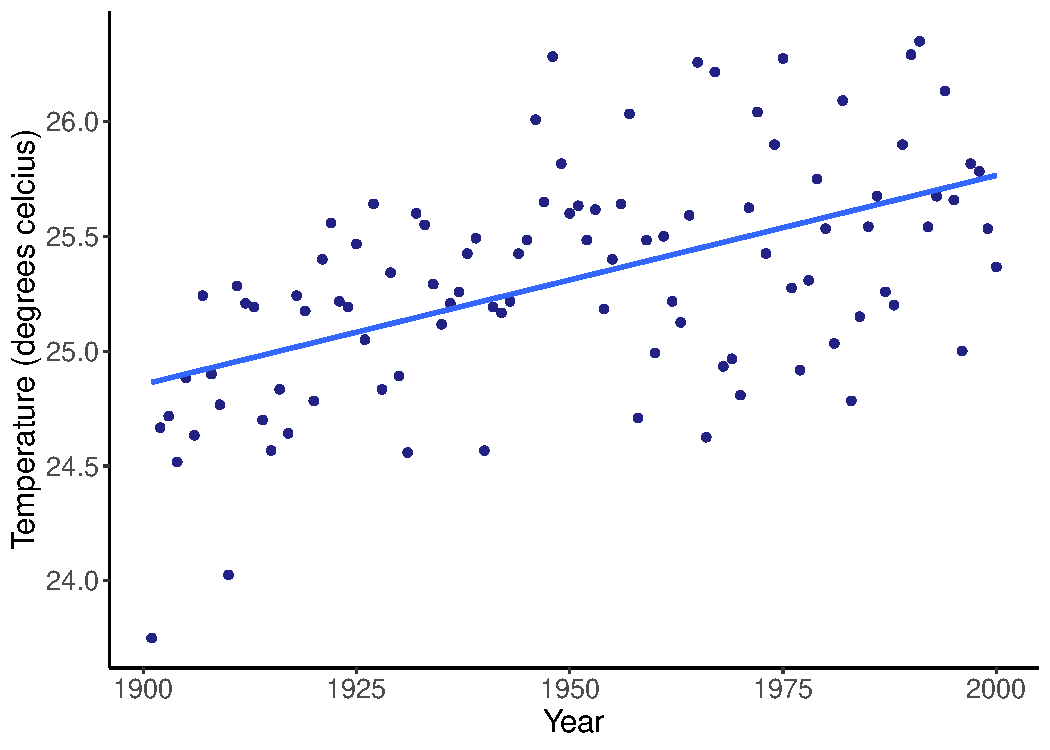
\includegraphics[width=0.8\textwidth, keepaspectratio]{../results/Temp_Year_florida.pdf}    
    \caption{The average annual temperatures in Florida from 1900 to 2000. The blue line illustrates the observed line of best fit over time.}
    \label{fig1}
  \end{figure}

    The observed calculated correlation coefficient (Pearson) for temperature and year was found to be 
    0.533 (t = 6.24, df = 98, p-value$<0.05$). Simulation results found that the mean correlation value obtained
    from simulations was 0.0005, with maximum and minimum values ranging from 0.31 to -0.30. Therefore, the 
    asymptotic p-value calculated was found to be 0. 

    \section*{Discussion}
    The results from this analysis, looking at the observed and simulation of randomized values, 
    show that the observed correlation between temperature and years in Florida are not obtained by chance 
    and that the null hypothesis should be rejected. There seems to be a moderate positive correlation between 
    temperature and increasing number of years, suggesting that temperatures seem to be rising in Florida.

\end{document}